\chapter{Conclusioni}
%\markboth{Introduzione}{Introduzione}
\label{cap:conclusioni}

\begin{figure}
\centering
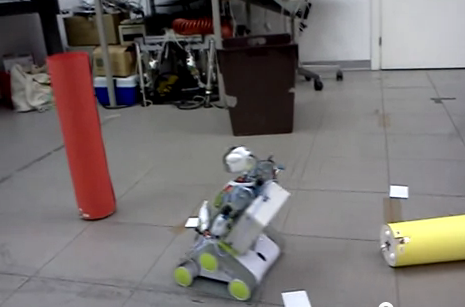
\includegraphics[scale=0.3]{images/attaccotorre}
\caption{Spykee va all'attacco della torre}
\end{figure}

Dalle prove che abbiamo effettuato, \emph{RoboTower} risulta giocabile e coinvolgente per il giocatore. Variando il numero e la dimensione degli ostacoli fissi, oppure agendo sui parametri di configurazione, quali la durata del singolo round oppure il tempo di ricarica delle carte, è possibile rendere il gioco più o meno difficile, e quindi adattarlo al giocatore. Agendo sulla dimensione del campo di gioco, invece, è possibile porre maggiormente l'accento sull'aspetto strategico del gioco (posizionamento corretto degli ostacoli, delle torri e delle fabbriche all'inizio del gioco), oppure su quello dinamico (posizionamento delle trappole durante l'avanzata del robot). Perché il gioco funzioni correttamente, comunque, il campo di gioco, deve avere una dimensione abbastanza piccola (ad esempio, un quadrato di lato $4$ m).

Le maggiori problematiche relative all'implementazione del gioco riguardano alcuni limiti degli strumenti a disposizione, in particolare del sistema di visione e del controllo del movimento. Per quanto riguarda la visione, il funzionamento degli algoritmi è fortemente inficiato dalla qualità dell'immagine proveniente dalla telecamera. Le immagini, infatti, a causa della forte compressione JPEG cui sono sottoposte, hanno visibili artefatti che influenzano negativamente il riconoscimento dei blob colorati. Purtroppo, essendo la compressione effettuata a bordo del robot, non è possibile ridurre la compressione. Altri problemi della visione sono legati alla forte dipendenza alle condizioni di luminosità dell'algoritmo di visione utilizzato, che rende necessario effettuare più volte il training del classificatore, a seconda delle condizioni di luce.

Per quanto riguarda il controllo del movimento, l'imprecisione dei comandi ricevuti dal robot e la strategia di controllo attuata (ad anello aperto) rendono impossibile controllarne l'effetto sull'attuale hardware. Questo provoca dipendenza della risposta del robot ai comandi da molteplici fattori, come la carica della batteria e la superficie su cui si muove. I frequenti ritardi nella trasmissione dei comandi, e il fatto che questi vengano eseguiti in coda, rendono difficile far agire il robot in maniera istantanea. A causa della mancanza di opportuni sensori, risulta impossibile creare una mappa dell'ambiente, o più semplicemente mantenere informazioni riguardo le posizioni di alcuni elementi rispetto al robot: questo non permette di attuare strategie complesse, che tengano conto della posizione degli oggetti già visti, e di pianificare in maniera adeguata l'aggiramento degli ostacoli.

I maggiori successi nell'implementazione del robot provengono dallo sfruttamento della logica fuzzy e da MrBrian, che ben si adattano a situazioni poco definite, come lo sono i dati che vengono estratti dai sensori del robot. Tramite regole fuzzy, si è riusciti a implementare un comportamento che risponde abbastanza bene agli stimoli dell'ambiente, rendendo il robot in grado di evitare ostacoli in maniera abbastanza soddisfacente e di puntare gli obiettivi seguendo delle traiettorie abbastanza pulite e razionali, nonostante il controllo impreciso dei motori.

Altri ottimi risultati sono arrivati grazie al middleware ROS, che ha consentito un forte disaccoppiamento delle parti del sistema, favorendo la riusabilità dei componenti. È facile quindi re-implementare parte del codice per portare RoboTower su altri robot. Inoltre, fornisce  moltissimi tool grafici e da linea di comando per semplificare il debug e il design delle applicazioni. 

%TODO accennare al riconoscimento giocatore x evitare che si metta davanti alla torre???

\section*{Ringraziamenti}

Ringraziamo Davide Perego per averci fornito le immagini, sia per gran parte delle carte, sia per il logo dell'interfaccia grafica del gioco RoboTower.

Un grosso ringraziamento va inoltre a tutto lo "staff" dell'AIRlab per il loro grandissimo supporto durante tutto lo svolgimento del progetto, in particolare il prof. Bonarini, Davide Rizzi e Martino Migliavacca: il loro aiuto ci è stato fondamentale!